%%============
%%  ** Author: Shepherd Qirong
%%  ** Date: 2021-12-20 22:40:58
%%  ** Github: https://github.com/ShepherdQR
%%  ** LastEditors: Shepherd Qirong
%%  ** LastEditTime: 2023-03-20 21:21:11
%%  ** Copyright (c) 2019--20xx Shepherd Qirong. All rights reserved.
%%============


\chapter{09-01-Introduction}
Today is 20211204, and I deciede to note down all of my knowledge about the math in this notebook.


数学史不单独作为一章,分布在各个章节中。

\section{Methodology}
方法论,数学重要思想。


\section{History}

\subsection{古代【公元前2000年-公元1689年】}


\subsubsection{古巴比伦和古埃及}

公元前3000年左右,巴比伦和埃及,数学出现。

有:整数和分数的算术、进制计数法、初步代数、几何经验公式。
无:成套记号、有意识的抽象思维、一般方法论、证明、直观推理。


\paragraph{古巴比伦}

巴比伦,美索不达米亚平原,公元前600年到公元300年间,泥板和楔形文字,公元前2000年左右的泥板也有部分保留下来。60进制,几个特殊的分数$\frac{1}{2},\frac{1}{3},\frac{2}{3}$有单独的记号。

算术,平方、平方根、立方、立方根表。
代数,$1^2 + 2^2 + \cdots + n^2$的公式。$x^2 + y^2 = 2z^2$的整数解。用特殊名称和记号表示未知量。
几何,特定等腰三角形的外接圆半径。计算简单平面图形和简单立体体积的方法。

【应用】

计算长度、重量,兑换钱币和交换商品,计算单利、复利、税收,分配粮食,划分土地、遗产。

月日观察的数据计算,计算相继数据之间的一次差分、二次查分。观察到这些差分等于常数时的情况,对数据做内插和外插。新月和亏蚀出现的时间计算误差在几分钟。恒星年(太阳相对恒星的位置复原所需要的时间)相差4.5分。

用阴历。每月在月球全黑(所谓的新月)后首次出现峨眉月开始,日子从出现峨眉月那天晚上开始计算,从日落到第二天日落之间算作一天。逐年算出夏至时间,定出冬至、春分、秋分。

算术、代数、几何的步骤是根据物理事实、不断试验和修改,从直观认识中得到的。


\paragraph{埃及}

埃及文化在公元前2500年左右达到顶峰,修建金字塔。到公元600年左右,埃及的历史和数学附属于希腊文明。

有多套文字:象形文字,用在碑文和器皿上;僧侣文,用于日常书写。

算术,单位分数。
代数,$ax^2 = b$。
几何,椎底是正方形的截棱锥体积$V = \frac{1}{3}(a^2+ab + b^2)$。


【应用】

计算报酬、谷仓容积、土地面积、天文历法。

观察天狼星计算太阳年,这颗星在夏季某一天可以在太阳快出来的时候在地平线上看到,称为天狼星的先阳升日,2个先阳升日之间相差365.25天,定一年为365天。尼罗河水开始上涨的那天定为一年第一天。起初定一年12个月,每月30天。在公元前45年,定一年为365.25天。



\subsubsection{古希腊}

公元前775年,将象形文字改为拼音字母。


\paragraph{古典时期【公元前600年-公元300年】}
Euclid的《几何原本》和Apollonius的《圆锥曲线》

Pythagoras学派开始,研究抽象概念。三角形数,沙滩上的小石子堆,求和公式。$1 + 2 + \cdots + n$的公式。

\begin{figure*}[h]
    \centering
    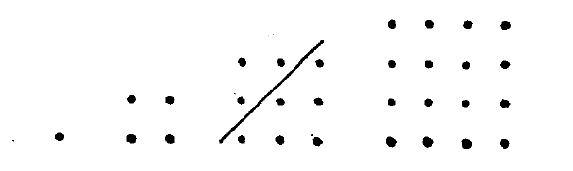
\includegraphics[width=0.5\textwidth]{./resources/古今数学思想-图3_2.png}
    \caption{[三角形数]}
    \label{fig:1}
\end{figure*}

\begin{figure*}[h]
    \centering
    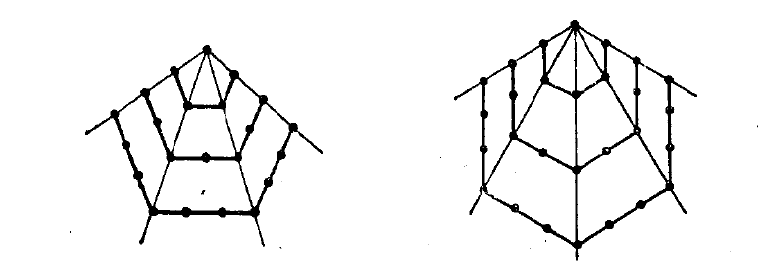
\includegraphics[width=0.5\textwidth]{./resources/古今数学思想-图3_5.png}
    \caption{[n边形数]}
    \label{fig:2}
\end{figure*}

Zeno生于公元前495到公元前480年间,当时人们对空间和时间有2种相对的看法,一是无限可分,运动是连续和平顺的;另一是由不可分的小段组成,运动是一系列小跳动。

Aristotle批判Zeno悖论:
悖论1,两分法悖论:从A到B,要先到之间的中点,空间无限可分,包含无限中点,不可能在有限时间内通过有限长度,若能通过,意味着必须到达没有终点的某种东西的终点。【Aristotle批,长度由无限点组成,时间段由无限时刻组成,有限时间段内可通过长度。】
悖论2,运动慢的不会被运动快的追上,因为要不断到达被追者前一刻所在的点。
悖论3,飞矢不动,任意瞬时必定在确定位置,因而是静止的。【Aristotle批,不承认时间具有不可分的单元。】
悖论4,A静止,一定时间内B左走1,C右走1,则B和C相差2。【速度是相对的,没有绝对的空间可以作为规定速度的依据】

Eudoxus证明了圆锥和棱锥的体积等于同底同高的圆柱和棱柱的三分之一。

Hippias,生于公元前460年左右,诡辩学派。


AB顺时针匀速转到AD,BC匀速运动到AD,交点从B逐渐运动到G。$\frac{\phi}{\pi *0.5} = \frac{E'H}{BA}$
\begin{figure*}[h]
    \centering
    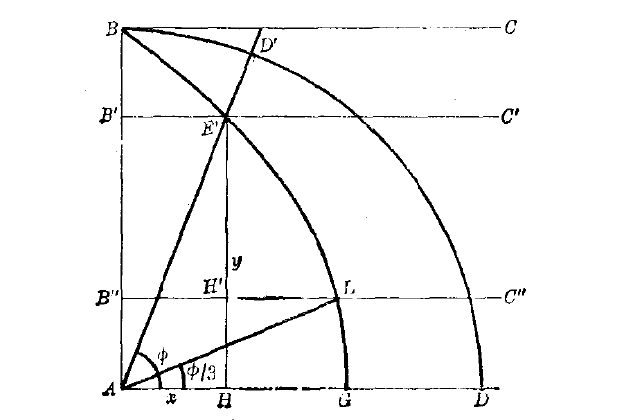
\includegraphics[width=0.5\textwidth]{./resources/古今数学思想-图3_10.png}
    \caption{[割圆曲线]}
    \label{fig:3}
\end{figure*}


\begin{figure*}[h]
    \centering
    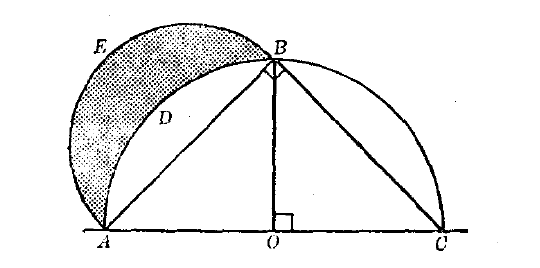
\includegraphics[width=0.5\textwidth]{./resources/古今数学思想-图3_11.png}
    \caption{[阴影面积=三角形AOB的面积]}
    \label{fig:4}
\end{figure*}

Plato学派。Archytas把曲线作为动点的轨迹,把曲面作为是曲线移动而产生的。Plato认为具体事物的完美理想才是实在,相信有一个独立、永恒的观念世界。从Plato开始要求根据公认的原理进行形式上的演绎证明。Plato学派字重要的发现是圆锥曲线。

\begin{figure*}[h]
    \centering
    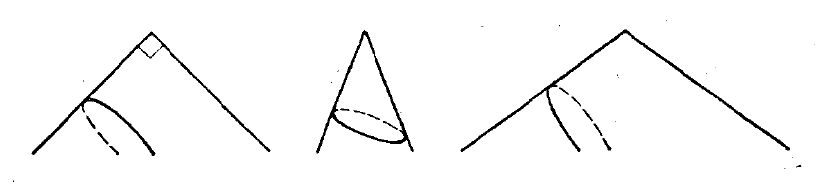
\includegraphics[width=0.5\textwidth]{./resources/古今数学思想-图3_12.png}
    \caption{[Menaechmus通过垂直于锥面的母线割锥面获得圆锥曲线]}
    \label{fig:5}
\end{figure*}

Endoxus引入变量的概念。建立了数学上以明确公理为依据的推演。

形而上学家研究数学家和自然哲学家(科学家)认为是不言而喻的东西,如研究对象的存在性、真实性问题、公理的本性问题。

Aristotle指出(据Plutarch 说 Plato较早指出过)一个定义只能告诉我们一件事物是什么,并不说明它一定存在.定义了的东西是否存在有待于证明,除非是少数几个第一性的东西诸如点和直线,它们的存在是同公理(第一性原理)一起事先为人们所接受的.

Aristotle和 Euelid所采取的用以证明存在性的方法是构造(construction).Euelid 《原本》中头三个公理承认直线和圆的构造;所有其他数学概念则必须构造出来以证明其存在,例如角的三等分线虽可定义,但不能用直线和圆构造出来,所以在希腊几何学里不能加以考虑.
Aristotle 也讨论数学的基本原理.他把公理和公设加以区别,认为公理是一切科学所公有的真理,而公设则只是为某一门科学所接受的第一性原理.他把逻辑原理(诸如矛盾律、排中律、等量加减等量后结果相等的公理以及其他这类原理)都列为公理.公设无需是不言自明的,但其是否属真应受所推出结果的检验.所列出的一批公理或公设,数目应该愈少愈好,只要它们能用以证明所有结果.

Aristotle讨论了怎样能把点同线联系起来这个基本问题.他说点不可分,然而占有位置.但那样的话,尽管聚集起多少点来,还总是聚不成能分的东西,而线段则肯定是能分的量.因此点不能形成象线这类连续的东西,因为点与点不能自己连续在-起.他说一点好比是时间中的“此刻”(现在).此刻不可分,因而并非时间的一部分.一点可能是一线的末端、开端或其上的分界处,但它不能是线的一部分,也不成其为量.一点只有通过运动才能产生一线从而成其为量的本原..他又论证说点没有长度,因此若--线由点组成,它将没有长度.同样,如果时间由瞬刻组成,那就没有整个的时段了:关于线所具有的连续性,他是这样定义的:如果一件东西的任何两个相继部分在其接触处的两个界限合而为一,这东西就是连续的.实际上Aristotle讲过许多次关于连续量的话,讲法都不一致.但他那个主张的实质是:点和数是离散量,必须同几何上的连续量区别开来.在算术上没有连续集合(连续统).至于就两门学科的关系来说,他认为算术(即数论)是更准确的,因为数比几何概念更易于抽象化.他又认为算术要先行于儿何,因为在考察三角形之前先需要有三这个数.

时间在两个方向上是潜在无穷的。


【Euclid的《几何原本》】

一线的两端是点。
从任一点到任一点做直线是可能的。【他假设线是唯一的】
把有限直线不断沿着直线延长是可能的。


延长AB到AF,延长AC到AG,使得BF=CG,由三角形全等,得到角3=角4,角5=角6,从而证明等腰三角形两底角相等。
\begin{figure*}[h]
    \centering
    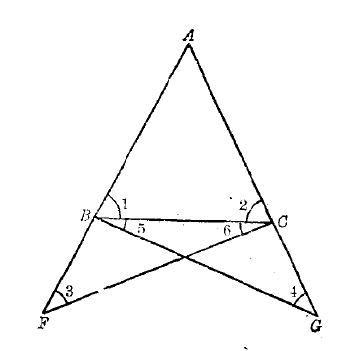
\includegraphics[width=0.5\textwidth]{./resources/古今数学思想-图4_2.png}
    \caption{[证明等腰三角形两底角相等]}
    \label{fig:6}
\end{figure*}

希腊人不承认无理数。

《几何原本》第5章,根据Eudoxus的工作写的“比例论”,是Euclid几何的最大成就。


求两数最大公度(公因子)的步骤. Euclid描述这个步骤的说法是:若A与B是两数且B<A,从4减去足够多次的B一直到余数О小于B.然后再从B减去足够多次的C直到余数小于C.这样一直做下去.若A与B互质,最后余数是1.那样1就是它们最大公因数.若A与B不互质,就会在某一阶段有最后一数量尽前一个数的情况.这最后的数便是A与的最大公因数.这种步骤现今称作Euclid算法.

可以每个顶点用3个正方形构成立方体,用3个正五边形构成正二十面体。

先给出一系列公理,然后推理。

对于无限远空间所必须成立的任何说法,其具体意义总是含糊不清的。【但是说两直线在有限远相交,但无法指出有限远在何处,是不是含糊不清呢?】

要假定移动图形而不改变图形的性质,需要对物理空间做很多限定。

两条直线可以相交但是没有公共点。




【Apollonius的《圆锥曲线》】



\begin{figure*}[h]
    \centering
    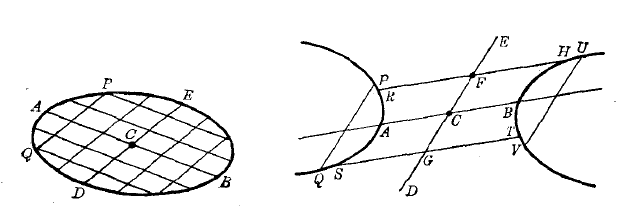
\includegraphics[width=0.5\textwidth]{./resources/古今数学思想-图4_21.png}
    \caption{弦中点}
    \label{fig:7}
\end{figure*}
椭圆中弦PQ,平行于弦PQ的所有弦的中点在一条直线上,记为AB。过AB的中点做弦DE平行于PQ,则DE上所有的点是平行于AB的弦的中点。


\begin{figure*}[h]
    \centering
    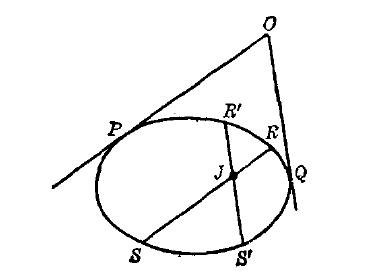
\includegraphics[width=0.5\textwidth]{./resources/古今数学思想-图4_26.png}
    \caption{【切线与面积】}
\end{figure*}\label{fig72}


【切线与面积】\ref{fig72}过O做圆锥曲线的两切线OP和OQ,做弦RS和$R'S'$分别平行于两切线,交点J,则有$ \frac{RJ*JS}{R'J*JS'} = \frac{OP^2}{OQ^2}$


\begin{figure*}[h]
    \centering
    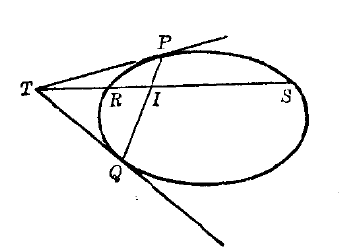
\includegraphics[width=0.5\textwidth]{./resources/古今数学思想-图4_27.png}
    \caption{【调和1】}\label{fig:7}
\end{figure*}
【调和1】$ \frac{TR}{TS} = \frac{IR}{IS}$


\begin{figure*}[h]
    \centering
    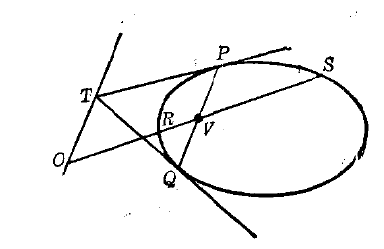
\includegraphics[width=0.5\textwidth]{./resources/古今数学思想-图4_28.png}
    \caption{【调和2】}\label{fig:7}
\end{figure*}
【调和2】$ \frac{OR}{OS} = \frac{VR}{VS}$


\begin{figure*}[h]
    \centering
    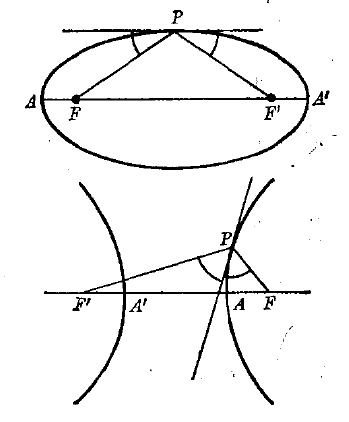
\includegraphics[width=0.5\textwidth]{./resources/古今数学思想-图4_29.png}
    \caption{【焦距】}\label{fig:7}
\end{figure*}
【焦距】圆锥曲线上点P与两焦点连线与切线交于等角。P与两焦点连线之和或差等于$A'A$

Euclid部分解决一个问题:与四根固定直线距离p,q,r,s,满足$pq = \alpha rs$,其中$\alpha$已知,求动点轨迹。Pappus也早知道这动点是圆锥曲线。

\paragraph{希腊时期【公元300年-公元600年】}



\subsection{近代【公元1689年-公元1917年】}


\subsection{现代【公元1917年-现在】}




\section{数学的思维方式与创新-84-北大(丘维声)}
6,1039. 

\subsection{数学史上的重大创新}


\subsubsection{分析:微积分的创立和完备化}
观察现象主要特征,抽象出概念。探索。猜测。证明。\\
如求瞬时速度, $s=at^2$,$\frac{\Delta s}{\Delta t}=2at+\Delta t$,牛顿忽略$\Delta t$,叫做留数,留下来的数。\\
如何解决不等于零又等于零的矛盾?\\
delta t 趋近于0,无限,柯西引入极限的概念:函数在x0附近有定义,在x0可以没有定义,如果存在c使得x趋近于x0但不等于x0时,$|f(x)-c|$可以无限小,称c是x趋近于x0时f(x)的极限。\\
$\forall \varepsilon >0,\ \exists \delta >0$, that when $0<|x-x_0|<\delta$, we have $|f(x)-c|<\varepsilon$
\subsubsection{几何:欧几里得几何到非欧几里得几何}
从平直空间到弯曲空间。\\
从定义和公理,推导和推演。平行公设。高斯和波约,罗巴切夫斯基(1829年),平行公设只是假设。现实世界如何实现非欧几何的用处。高斯想法把球面本身看做一个空间。后来黎曼发展了。弯曲空间的几何是黎曼几何,如球面上的直线定义为大圆的一部分,这样发现过已知直线外一点不存在其平行线。在双曲几何模型下可以实现罗巴切夫斯基几何。\\
\subsubsection{代数学中}
伽瓦罗,代数学从研究方程的根,到研究代数系统的结构和保持运算的映射。

\subsection{集合的划分}
交空并全的划分方法:模n同余是$\mathbb Z$的一个二元关系。两个集合的笛卡尔积\\
a与b模n同余:$(a,b) \in \bigcup _{i=0}^{n-1} H_i \times H_i \subseteq \mathbb Z \times \mathbb Z$.抽象:非空集合s,$S\times S$的子集W是S是上的二元关系,有关系的记为aWb\\

\subsubsection{等价关系}
反身性,对称性,传递性,$a \sim b$. $a \sim b \Leftrightarrow b \sim a$. $a \sim b , b \sim c \Rightarrow a \sim c$\\
$\bar a$ 是a确定的等价类,$\left\{ x \in S |x \sim a \right\}$。易有
$\bar x = \bar y \Leftrightarrow x \sim y$ 。\\


定理1:集合S上等价关系$\sim$给出的等价类的集合是S的一个划分。\\
证明思路:需要证明并全,交空。交空比较难,需要研究等价类的性质。等价类的代表不唯一。\\
Step1)  It is obvious that $\cup _{a \in S} {\bar a} \subseteq S$,and for any $b \in S$, we have $b \in \bar b \in \cup _{a \in S} {\bar a}$, this means $S \subseteq \cup _{a \in S} {\bar a}  $, so $ \cup _{a \in S} {\bar a} =S $.\\
Step2) To prove $\bar x \neq \bar y \Rightarrow \bar x \bigcap \bar y = \varnothing  $, we prove the contrapositive $ \bar x \bigcap \bar y \neq \varnothing \Rightarrow  \bar x = \bar y$, and this is easy to prove.\\







\section{Space}

\subsection{Operation Defination}

\subsubsection{Element}

we define the basic element as following, where $ \boldsymbol e_i $ means $x_i = 1, x_j = 0$ for all $j \neq i$. When we say a vector, we normally mean a column vector.

\begin{equation}
\vec{x}  = \boldsymbol x = [x_1, x_2,\dots]^T
= \begin{bmatrix}
    x_1 \\
    \vdots \\
    x_n
\end{bmatrix}
= \Sigma x_i \boldsymbol{e_i} 
\end{equation}

We define Kronecker sign to simply the description of $\boldsymbol e_i \cdot \boldsymbol e_j $.

\begin{equation}
    \begin{split}
    &\delta _{ij}:=
    \begin{cases}
    &1,\qquad i = j\\
    &0,\qquad i \neq j\\
    \end{cases}\\
    \end{split}
\end{equation}

The set of bases $\{ \boldsymbol e_i  \}  \xrightarrow{apply} \boldsymbol{x} \longrightarrow    \{ x_i \}   $.
%%\stackrel{apply}
%%\xrightarrow[under]{up} 


\subsubsection{Dot Product}

We define in algebra, $ \boldsymbol{x} \cdot \boldsymbol{y} := \sum{x_iy_i \delta _{ij}} = \boldsymbol{x}^T \cdot \boldsymbol{y}$.

Then the defination is restricted to the choose of the coordinate system. We take a look a the product with reflect $T : \boldsymbol x \rightarrow  \boldsymbol{T} \cdot \boldsymbol{x}$,

\begin{equation}
    (\boldsymbol A \cdot \boldsymbol  B)^T = (a_{ik}b_{kj})^T = c_{ij}^T = c_{ji} = b_{jk}a_{ki} = \boldsymbol B^T \cdot \boldsymbol A^T
\end{equation}
we have 
\begin{equation}
    (\boldsymbol T \cdot \boldsymbol  x)^T(\boldsymbol T \cdot \boldsymbol  y) =  \boldsymbol x^T (\boldsymbol T^T \boldsymbol T) \boldsymbol y = [(\boldsymbol T^T \boldsymbol T) \boldsymbol x]^T \boldsymbol y
\end{equation}

We name T a Contractive mapping when $\boldsymbol T^T \boldsymbol T \leqslant   \theta, 0 \leqslant \theta \leqslant 1$.

\subsubsection{geometry Properties}

\begin{equation}
    \begin{split}
    &\parallel \boldsymbol{x} \parallel := \sqrt{\boldsymbol x \cdot \boldsymbol x}\\
    &\cos {\theta_{x,y}} : = \frac
    {\boldsymbol x \cdot \boldsymbol x}
    {\parallel \boldsymbol{x} \parallel \cdot \parallel \boldsymbol{y} \parallel}\\
\end{split}
\end{equation}

\subsubsection{Add}

\begin{equation}
    \begin{split}
    & \boldsymbol x + \boldsymbol y := \sum (x_i + y_i)\boldsymbol e_i\\
    & k \cdot \boldsymbol x := \sum kx_i\boldsymbol e_i\\
\end{split}
\end{equation}

Law $\boldsymbol{x} + \boldsymbol{y} = \boldsymbol{y} + \boldsymbol{x}$,
law $ (\boldsymbol{x} + \boldsymbol{y} )+ \boldsymbol{z} = \boldsymbol{x} +( \boldsymbol{y} + \boldsymbol{z})$ is not obvious in the view of Set Theory.




\section{Euclid空间}
有序的n元组的全体称为n维Euclid空间,记为$\mathbb R^n$,称$\boldsymbol p=(p_i)_{i=1}^n \in \mathbb R^n$是$\mathbb R^n$的一个点。\\
为便于研究,本论文以$ \mathbb R^3$为背景空间,所涉及的函数默认为可微实值函数。如果实函数$f$的任意阶偏导数存在且连续,则称函数是可微的(或无限可微的,或光滑的,或$C^\infty$的)。\\
由于微分运算是函数的局部运算,限制所讨论函数的定义域在$ \mathbb R^3$中的任意开集,所讨论的结论仍然成立。\\
自然坐标函数:定义在$\mathbb R^n$上的实值函数$x_i: \mathbb R^n \to  \mathbb R$,使得$\boldsymbol p=(p_i)_{i=1}^n = \left( x_i(\boldsymbol p) \right)_{i=1}^n   $\\
切向量:由$\mathbb R^n$ 中的二元组构成,$\boldsymbol v_{\boldsymbol p}=(\boldsymbol p,\boldsymbol v)$,其中$\boldsymbol p$是作用点,$\boldsymbol v$是向量部分\\
切空间$T_p  \mathbb R^n$: 作用点$\boldsymbol p \in \mathbb R^n$的所有切向量的集合。利用向量加法与数量乘法使某点的切空间称为向量空间,与背景空间存在非平凡同构。\\
向量场$\boldsymbol V$:作用于空间点的向量函数,$\boldsymbol V(\boldsymbol p)\in T_p  \mathbb R^n $\\
逐点化原理:$(\boldsymbol V+\boldsymbol W)(\boldsymbol p)=\boldsymbol V(\boldsymbol p)+\boldsymbol W(\boldsymbol p),\ (f \boldsymbol V)(\boldsymbol p)= f(\boldsymbol p)\boldsymbol V (\boldsymbol p)$\\
自然标架场:定义$\boldsymbol U_i=(\delta _j^i)_{j=1}^n$,按Einstein求和约定,有$\boldsymbol V(\boldsymbol p)=v^i(\boldsymbol p)\boldsymbol U_i(\boldsymbol p)$,称$v^i$为场的Euclid坐标函数,其中Kronecker $\delta$函数定义为:
\begin{equation}
\label{Kronecker_delta}
\delta _i^j=\left\{ 
    \begin{aligned}
    1,\  & i =j\\
    0,\  & i \neq j\\
    \end{aligned}
     \right.
\end{equation}

\section{Reference}







